\setchapterpreamble{
    \lettrine{I}{n}~the flavour sector of the Standard~Model, particle interaction eigenstates are not equal to their mass eigenstates.
    This phenomenon has many interesting consequences, including meson mixing and \CP~violation.
    This~\lcnamecref{chp:theory} discusses those consequences for select physics processes.}

\chapter{Theory}
\label{chp:theory}

\vspace*{\fill}
\minitoc

\clearpage
\section{Particles and interactions}
\label{sec:SM}

The Standard Model of particle physics~(SM) uses a small number of particles, depicted in \cref{fig:theory_SM_Particles}, to describe nature at the smallest scales.
Firstly, matter is implemented in the model as the spin-\(\sfrac{1}{2}\)~fermions.
Secondly, the spin-1~bosons are based on gauge symmetries, and act as force-carriers.
Finally, the scalar Higgs~field generates the mass of these particles.

The~SM implements three fundamental forces:
%
\begin{figure}[b] \centerfloat
    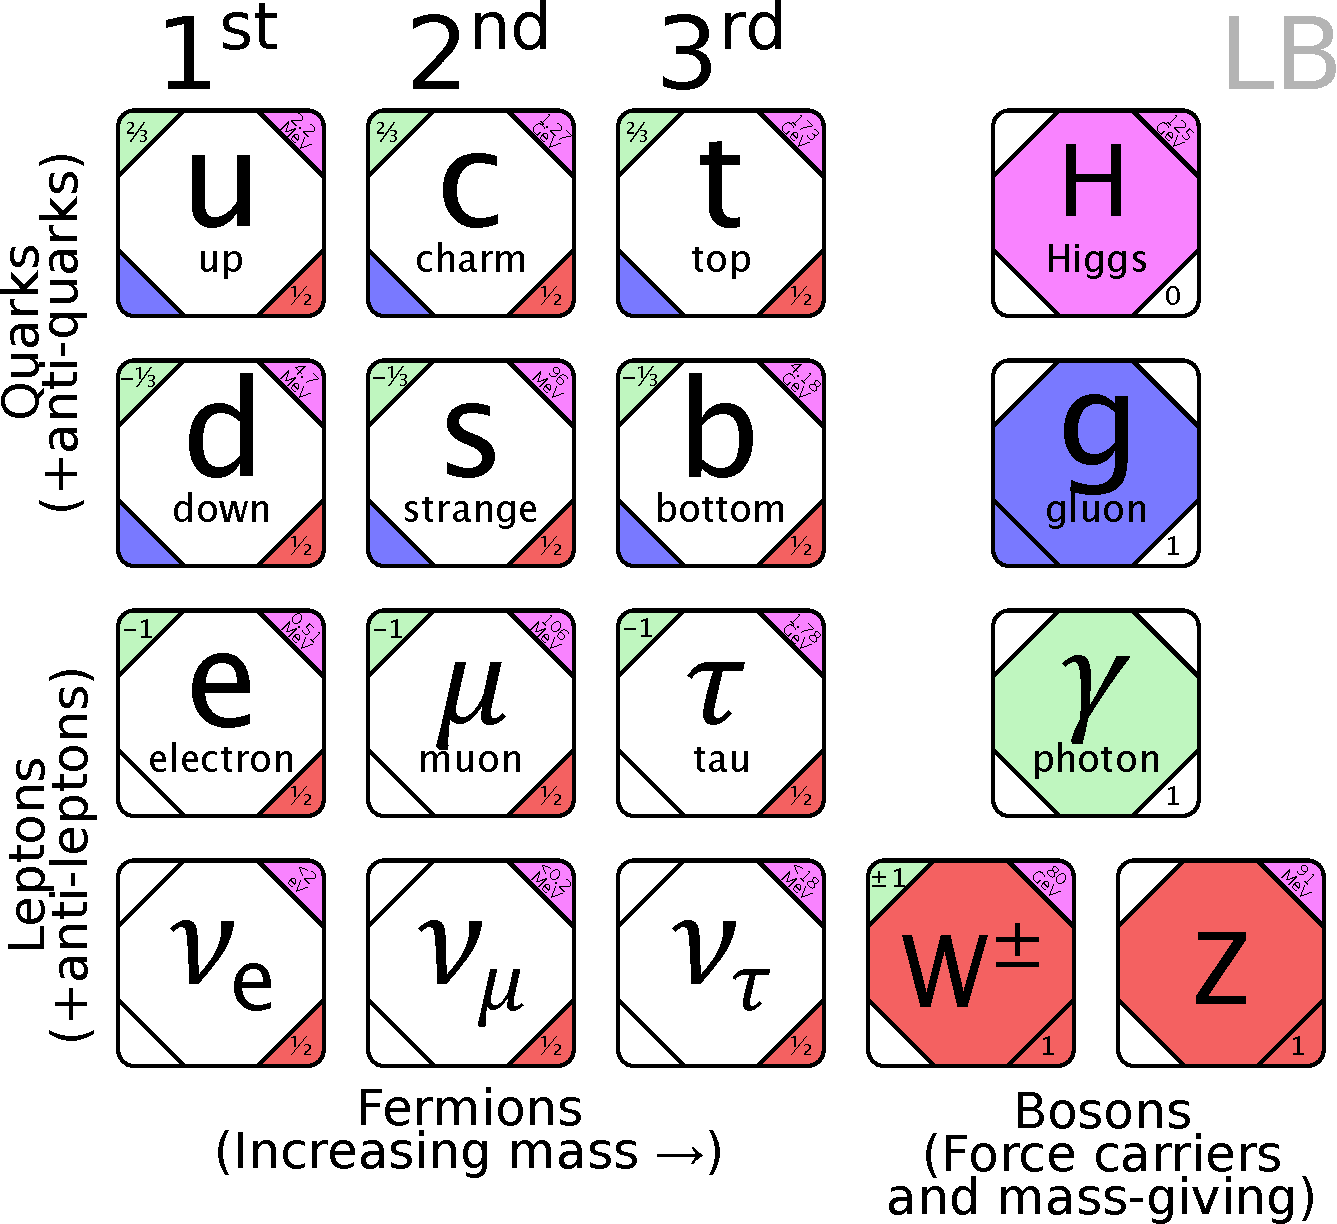
\includegraphics[width=\textwidth]{theory/SM}
    \caption{
        The various particles of the Standard~Model of particle~physics, with fermions on the left and bosons on the right.
        In each box several properties are denoted: electric~charge in the top-left~corner, mass in the top-right~corner, presence or absence of colour in the lower-left~corner, and weak~isospin in the lower-right~corner.}
    \label{fig:theory_SM_Particles}
\end{figure}
%
\begin{itemize}
    \item The electromagnetic force, mediated by the photon~(\g). This force acts upon any charged particle, including the six quarks, the three charged leptons, and the \Wpm~bosons.
    \item The weak force, mediated by the \Wpm~and \Z~bosons. This force acts upon isospin-charged particles, including all the fermions, and the \Wpm~and \Z~bosons themselves.
    \item The strong force, mediated by the gluons~(\gluon). This force acts upon colour-charged particles: the six quarks, as well as the gluons themselves.
\end{itemize}

The~SM describes both ordinary matter and its counterpart, antimatter.
Fundamentally, the theory requires that matter and corresponding antimatter particles have the same mass and lifetime.
Furthermore, electromagnetic and strong interactions are symmetric for matter and antimatter particles.
This symmetry is \CP~symmetry, where \CP~is defined as the successive application of two discrete symmetries: charge conjugation~\(C\) and the parity inversion~\(P\).
The \(C\)~operation transforms particles into antiparticles and vice versa, while the \(P\)~operation transforms \({\left(x, y, z\right)}\)~coordinates into~\({-\left(x, y, z\right)}\), and therefore interchanges left- and right-handed particles.

In the Standard~Model, parity violation is described by introducing a weak force gauge symmetry only for left-handed particles and right-handed antiparticles.
\CP~violation in the~SM, a subtle manifestation of which was discovered in~1964~\cite{CPinKaon}, is possible due to complex interaction couplings in the weak interaction.
The origin of this lies in the fact that the weak interaction eigenstates of the fermions are not identical to the mass eigenstates.

\clearpage
\section{The CKM~matrix}
\label{sec:CKM}

In the Standard Model Lagrangian, the mass terms of the quark fields arise from the Yukawa couplings between the quarks and the Higgs field,
%
\begin{equation}
    \Lagrangian_{\text{Yukawa}}^{\text{quarks}} = Y_{ij}^{d} \overline{Q_{\text{L},i}^{\text{I}}} \phi d_{\text{R},i}^{\text{I}} + Y_{ij}^{u} \overline{Q_{\text{L},i}^{\text{I}}} \tilde{\phi} u_{\text{R},i}^{\text{I}} \text{h.c.} \rlap{,}
\end{equation}
%
with the Yukawa~couplings~\(Y\) between the Higgs~doublets~\(\phi\) and~\(\tilde{\phi}\), the left-handed quark doublets~\(Q_{\text{L}}^{\text{I}}\), and the right-handed quark fields~\(d_{\text{R}}^{\text{I}}\) and~\(u_{\text{R}}^{\text{I}}\).
The label~I denotes expression in the interaction basis.
After spontaneous symmetry breaking~\cite{PhysRevLett.13.321,PhysRevLett.13.508}, the doublets are split, and the Yukawa couplings give rise to the quark mass terms,
%
\begin{equation}
    \Lagrangian_{\text{Yukawa}}^{\text{quarks}} = v Y_{ij}^{d} \overline{d_{\text{L},i}^{\text{I}}} d_{\text{R},i}^{\text{I}} + v Y_{ij}^{u} \overline{u_{\text{L},i}^{\text{I}}} u_{\text{R},i}^{\text{I}} + \text{h.c.} \rlap{,}
\end{equation}
%
where \({v = \SI{246}{\GeV}}\)~is the vacuum expectation value.
The interactions between the Higgs~boson and the quark fields have been omitted for brevity.

The Lagrangian of the charged-current interaction,
%
\begin{equation}
    \Lagrangian_{\text{cc}}^{\text{quarks}} = \dfrac{g}{\sqrt{2}} \left[ \overline{u_{\text{L},i}^{\text{I}}} \gamma_{\mu} \dfrac{1 - \gamma^{5}}{2} W^{-}{}^{\mu} d_{\text{L},i}^{\text{I}}
        + \overline{d_{\text{L},i}^{\text{I}}} \gamma_{\mu} \dfrac{1 - \gamma^{5}}{2}  W^{+}{}^{\mu} u_{\text{L},i}^{\text{I}} \right] \rlap{,}
\end{equation}
%
can be rewritten with the quark interaction fields in their mass eigenstates.
This requires diagonalisation of the matrix of Yukawa couplings, leading to
%
\begin{equation}
    \Lagrangian_{\text{cc}}^{\text{quarks}} = \dfrac{g}{\sqrt{2}} \left[
          \overline{u_{\text{L},i}} V_{\text{L}}^{u} \gamma_{\mu} \dfrac{1 - \gamma^{5}}{2} W^{-}{}^{\mu} V_{\text{L}}^{d}{}^{\dagger} d_{\text{L},i}
        + \overline{d_{\text{L},i}} V_{\text{L}}^{d} \gamma_{\mu} \dfrac{1 - \gamma^{5}}{2} W^{+}{}^{\mu} V_{\text{L}}^{u}{}^{\dagger} u_{\text{L},i}
    \right] \rlap{,}
\end{equation}
%
where the unitary matrices~\(V_{\text{L}}^{u}\) and~\(V_{\text{L}}^{d}\) diagonalise the matrix of up- and down-type quarks, respectively.

The interaction eigenstates can now be related to the mass eigenstates through the complex, unitary~\num{3x3} CKM~matrix~\({\VCKM = V_{\text{L}}^{u} V_{\text{L}}^{d}{}^{\dagger}}\), named after Cabibbo, Kobayashi and Maskawa,~\cite{CKM1,CKM2}
%
\begin{equation} \label{eqn:theory_CKM_Matrix}
    \begin{pmatrix}
        \dquark^{\text{I}} \\
        \squark^{\text{I}} \\
        \bquark^{\text{I}}
    \end{pmatrix}
    =
    \VCKM
    \begin{pmatrix}
        \dquark \\
        \squark \\
        \bquark
    \end{pmatrix}
    =
    \begin{pmatrix}
        \Vud & \Vus & \Vub \\
        \Vcd & \Vcs & \Vcb \\
        \Vtd & \Vts & \Vtb
    \end{pmatrix}
    \begin{pmatrix}
        \dquark \\
        \squark \\
        \bquark
    \end{pmatrix} \rlap{.}
\end{equation}
%
These nine complex numbers~\(\V{ij}\) define the relative values of the charged-current couplings in which a quark changes flavour.
The only interaction allowing flavour changes in the~SM is the weak interaction, through the charged \Wpm~bosons.
Under the \CP~transformation, each CKM~element changes into its complex conjugate, and thus it is the complex phases of the elements that can yield \CP~violation in the SM.

Since the CKM~elements only enter at the amplitude level, a single Feynman diagram can never yield measurable \CP~violation: the observable quantity, the magnitude of the amplitude, is then identical for the \CP-conjugate process.
Therefore, a prerequisite for observing \CP~violation is the interference between two amplitudes of comparable magnitude and with a different weak phase.
The complex phase of the weak interaction (known as the ``weak~phase'') will change sign under the \CP~transformation.
Measuring the difference in decay-rate between a process and its \CP-conjugate allows the determination of the phase difference between them, and hence of the weak phase difference and the amount of \CP~violation in that process.

To conserve total probability, the CKM~matrix must be unitary:~\({\VCKM\VCKMd = \VCKMd\VCKM = \identitymatrix}\).
This results in the following unitarity relations between the elements of the matrix:
%
\begin{subequations} \label{eqn:theory_CKM_Unitarity}
    \begin{align}
        \sum_{k} \V{ik} \Vs{jk} &= 0 \rlap{,} \label{eqn:theory_CKM_Unitarity_1} \\
        \sum_{k} \abs{\V{ik}}^{2} = \sum_{k} \abs{\V{ki}}^{2} &= 1 \rlap{,} \label{eqn:theory_CKM_Unitarity_2}
    \end{align}
\end{subequations}
%
for any two generations~\({i, j \in \{ u, c, t \}}\),~\({i \neq j}\).
From the original \num{18}~degrees of freedom of the matrix, these constraints leave a total of five relative quark field phases and four free parameters with which the matrix can be fully described: three angles and one complex phase.
Hence, the entirety of measurable \CP~violating phenomena in the~SM is reduced to a single parameter: the complex phase of the CKM~matrix.
It is noteworthy that this phase only appears in the case of at least three generations, making the~SM the minimal model with \CP~violation in the weak interaction.

The four parameters of the CKM~matrix are in principle free parameters of the Standard~Model, but they have been experimentally determined to show an interesting pattern.
The magnitudes of the diagonal elements are all close to unity, while the off-diagonal terms are smaller the greater the difference between the generations.
A common way of parameterising the matrix that exploits this structure is the Wolfenstein parameterisation~\cite{Wolfenstein:1983yz}.
This parameterisation consists of three real variables~\wolfl, \wolfA, and \wolfrho and one imaginary part \({i\wolfeta}\).
By construction, \({\wolfl = \sin(\theta_{\text{c}}) \approx 0.225}\)~\cite{CKM1}, naturally leading to an expansion in powers of~\wolfl.
Up to \({\order(\wolfl^{4})}\), the matrix takes the form
%
\begin{equation} \label{eqn:theory_CKM_Wolfenstein}
    \VCKM
    =
    \begin{pmatrix}
        1 - \frac{1}{2}\wolfl^{2} - \frac{1}{8}\wolfl^{4} & \wolfl & \wolfA\wolfl^{3}(\wolfrho - i\wolfeta) \\[.5ex]
        -\wolfl & 1 - \frac{1}{2}\wolfl^{2} - \frac{1}{8}\wolfl^{4}(1 + 4\wolfA^{2}) & \wolfA\wolfl^{2} \\[.5ex]
        \wolfA\wolfl^{3} (1 - \wolfrho - i\wolfeta) & -\wolfA\wolfl^{2} + \frac{1}{2}\wolfA\wolfl^{4}(1 - 2(\wolfrho + i\wolfeta)) & 1 - \frac{1}{2}\wolfA^{2}\wolfl^{4}
    \end{pmatrix} \rlap{.}
\end{equation}
%
Written in this form, the diagonal elements are recognised as a small deviation from unity, while the off-diagonal elements are all smaller with certain powers of~\wolfl.
The current world-average experimental determination of the parameters is~\cite{HFLAV2016}
%
\begin{subequations}
    \begin{align}
        \wolfl    &= {0.22543 }_{-0.00031}^{+0.00042} \\
        \wolfA    &= {0.8227\0}_{-0.0136}^{+0.0066} \\
        \wolfrhob &= {0.1504\0}_{-0.0062}^{+0.0121} \\
        \wolfetab &= {0.3540\0}_{-0.0076}^{+0.0069}
    \end{align}
\end{subequations}
%
where~\({\wolfrho + i\wolfeta}\) of \cref{eqn:theory_CKM_Wolfenstein} has been substituted by~\({\wolfrhob + i\wolfetab}\), defined as
%
\begin{equation} \label{eqn:theory_CKM_rhob_etab}
    \wolfrhob + i\wolfetab = -\dfrac{\Vud\Vubs}{\Vcd\Vcbs} = \dfrac{\sqrt{1-\wolfl^{2}} (\wolfrho + i\wolfeta)}{\sqrt{1 - \wolfA^{2}\wolfl^{4}} + \sqrt{1 - \wolfl^{2}}\wolfA^{2}\wolfl^{4}(\wolfrho + i\wolfeta)} \rlap{.}
\end{equation}

The six relations in \cref{eqn:theory_CKM_Unitarity_1} can be visualised as triangles in the complex plane, allowing verification of the compatibility of various measurements by checking that the triangles close.
The most pronounced unitarity triangle~(UT) is shown in \cref{fig:theory_CKM_UTBd}, with its apex at~\({\wolfrhob + i\wolfetab}\), justifying the definition in \cref{eqn:theory_CKM_rhob_etab}.
While the individual phases of the CKM~elements are not physical observables, certain combinations of phases are measurable quantities.
Those combinations show up in the UTs as the angles \CPalpha, \CPbeta, \CPgamma, and~\betas, as shown in \cref{fig:theory_CKM_UT}.
Additionally, the surface area of each UT is equal to \(\sfrac{1}{2}\)~the Jarlskog invariant~\Jarlskog,~\cite{PhysRevLett.55.1039}
%
\begin{equation} \label{eqn:theory_CKM_Jarlskog}
    \Jarlskog = \wolfl^{6}\wolfA^{2}\wolfeta \approx \num{3e-5}\rlap{.}
\end{equation}
%
The Jarlskog invariant is a measure of the amount of \CP~violation in the SM.

This thesis describes a measurement of~\weak, with \({\CPgamma = \arg\left(-\dfrac{\Vud\Vubs}{\Vcd\Vcbs}\right)}\) and~\({\betas = \arg\left(-\dfrac{\Vts\Vtbs}{\Vcs\Vcbs}\right)}\).
Using external input for~\betas from \BsToJPsiPhi~decays~\cite{HFLAV2016}, a determination of~\CPgamma is made, one the least-precise known observables constraining the apices of the UTs.
It should be noted that, in the Wolfenstein parameterisation up to~\({\order(\wolfl^{4})}\), \CPgamma~is given by the phase of~\Vub, \({\CPgamma \approx -\arg(\Vub)}\).

\begin{figure}[p] \centerfloat
    \begin{subfigure}{\textwidth} \centerfloat
        \begin{tikzpicture}
            \node[anchor=south west,inner sep=0] (image) at (0,0) {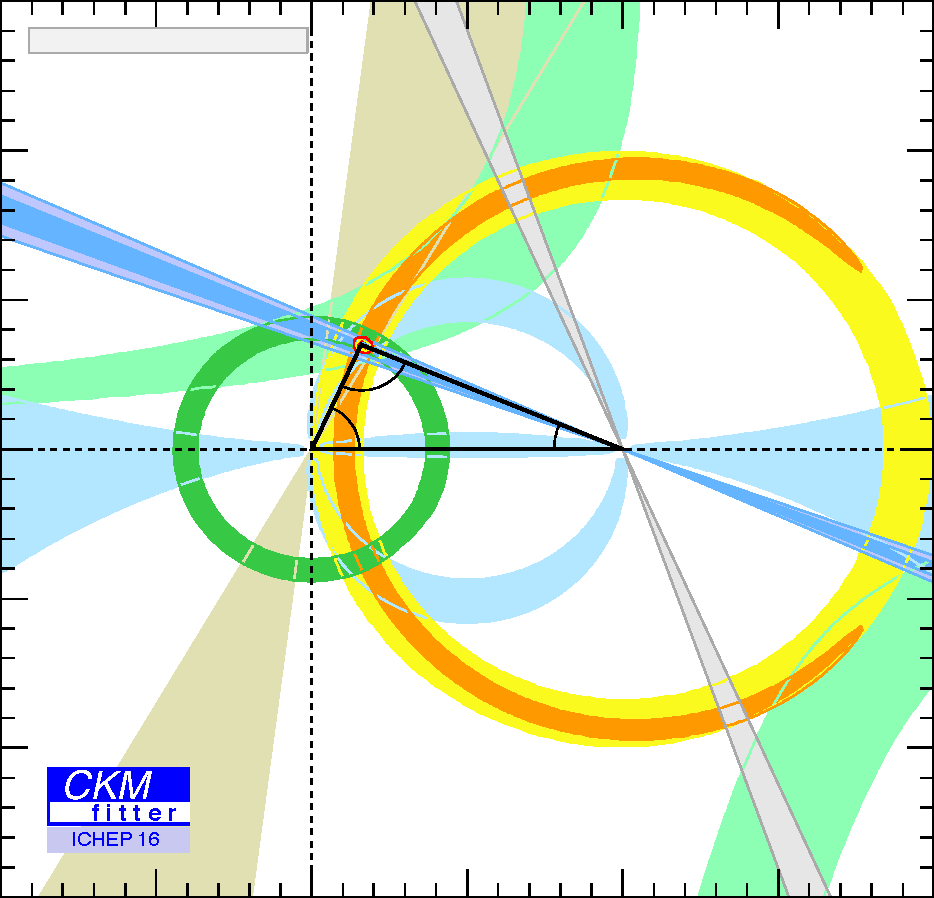
\includegraphics[width=0.55\textwidth]{theory/rhoeta_large}};
            \begin{scope}[x={(image.south east)},y={(image.north west)}]
                \node at (1. / 6. - 0.02, -0.027) {\(\pgfmathprintnumber[fixed,precision=1,fixed zerofill=true]{-0.5}\)};
                \foreach \x in {0, 2, 3, ..., 6}
                {
                    \tikzmath{\xpos = \x / 6.; \xtext = \x * 0.5 - 1.0;}
                    \node at (\xpos, -0.027) {\(\pgfmathprintnumber[fixed,precision=1,fixed zerofill=true]{\xtext}\)};
                }
                \node[anchor=east] at (0.005, 0.008) {\(\pgfmathprintnumber[fixed,precision=1,fixed zerofill=true]{-1.5}\)};
                \foreach \y in {1, ..., 6}
                {
                    \tikzmath{\ypos = \y / 6.; \ytext = \y * 0.5 - 1.5;}
                    \node[anchor=east] at (0.005, \ypos) {\(\pgfmathprintnumber[fixed,precision=1,fixed zerofill=true]{\ytext}\)};
                }

                {
                    \fontsize{4}{4.8}\selectfont
                    \node[anchor=west] at (0.04, 0.955) {excluded area has \({\text{CL} > \num{0.95}}\)};
                    \node[anchor=west,rotate=-68] at (0.475, 0.995) {excluded at \({\text{CL} > \num{0.95}}\)};
                    \node[anchor=west] at (0.76, 0.08) {sol. w/ \({\cos 2\CPbeta < 0}\)};
                    \node[anchor=west] at (0.76, 0.05) {(excl. at \({\text{CL} > \num{0.95}}\))};
                }
                {
                    \fontsize{10}{12}\selectfont
                    \node[anchor=west] at (0.40, 0.885) {\CPgamma};
                    \node[anchor=west] at (0.665, 0.810) {\dmd~\&~\dms};
                    \node[anchor=west] at (0.02, 0.730) {\({\sin 2\CPbeta}\)};
                    \node[anchor=west] at (0.82, 0.630) {\dmd};
                    \node[anchor=west] at (0.03, 0.575) {\epsK};
                }
                {
                    \fontsize{7}{8.4}\selectfont
                    \node[anchor=west] at (0.365, 0.580) {\CPalpha};
                    \node[anchor=west] at (0.530, 0.519) {\CPbeta};
                    \node[anchor=west] at (0.34, 0.514) {\CPgamma};
                }
                {
                    \fontsize{10}{12}\selectfont
                    \node[anchor=west] at (0.03, 0.460) {\CPalpha};
                    \node[anchor=west] at (0.175, 0.390) {\abs{\Vub}};
                    \node[anchor=west] at (0.59, 0.390) {\CPalpha};
                    \node[anchor=west] at (0.205, 0.165) {\CPgamma};
                    \node[anchor=west] at (0.86, 0.190) {\epsK};
                }

                \node[anchor=east] at (1.0, -0.10) {\wolfrhob};
                \node[rotate=90,anchor=east,inner xsep=0pt,outer xsep=0pt] at (-0.12, 1.0) {\wolfetab};
            \end{scope}
        \end{tikzpicture}
        \caption{The best-known Unitarity~Triangle, corresponding to \({\Vud\Vubs + \Vcd\Vcbs + \Vtd\Vtbs = 0}\). Its apex is at the point given in \cref{eqn:theory_CKM_rhob_etab}.}
        \label{fig:theory_CKM_UTBd}
    \end{subfigure}
    \begin{subfigure}{\textwidth} \centerfloat
        \begin{tikzpicture}
            \node[anchor=south west,inner sep=0] (image) at (0,0) {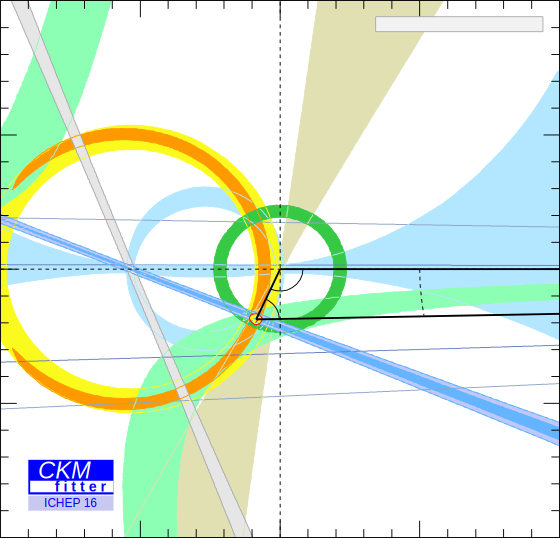
\includegraphics[width=0.55\textwidth]{theory/rhoetaBs_large}};
            \begin{scope}[x={(image.south east)},y={(image.north west)}]
                \node at (1. / 4. - 0.02, -0.027) {\(\pgfmathprintnumber[fixed,precision=1,fixed zerofill=true]{-0.05}\)};
                \foreach \x in {0, 2, 3, 4}
                {
                    \tikzmath{\xpos = \x / 4.; \xtext = \x * 0.05 - 0.10;}
                    \node at (\xpos, -0.027) {\(\pgfmathprintnumber[fixed,precision=2,fixed zerofill=true]{\xtext}\)};
                }
                \node[anchor=east] at (0.005, 0.010) {\(\pgfmathprintnumber[fixed,precision=2,fixed zerofill=true]{-0.10}\)};
                \foreach \y in {1, ..., 4}
                {
                    \tikzmath{\ypos = \y / 4.; \ytext = \y * 0.05 - 0.10;}
                    \node[anchor=east] at (0.005, \ypos) {\(\pgfmathprintnumber[fixed,precision=2,fixed zerofill=true]{\ytext}\)};
                }

                {
                    \fontsize{4}{4.8}\selectfont
                    \node[anchor=west] at (0.677, 0.955) {excluded area has \({\text{CL} > \num{0.95}}\)};
                    \node[anchor=west,rotate=-68] at (0.04, 0.995) {excluded at \({\text{CL} > \num{0.95}}\)};
                    \node[anchor=west] at (0.752, 0.465) {\betas};
                }
                {
                    \fontsize{10}{12}\selectfont
                    \node[anchor=west] at (0.090, 0.945) {\epsK};
                    \node[anchor=west] at (0.560, 0.925) {\CPgamma};
                    \node[anchor=west] at (0.180, 0.730) {\dmd~\&~\dms};
                    \node[anchor=west] at (0.010, 0.605) {\dmd};
                    \node[anchor=west] at (0.243, 0.590) {\CPalpha};
                    \node[anchor=west] at (0.504, 0.600) {\abs{\Vub}};
                    \node[anchor=west] at (0.868, 0.575) {\CPalpha};
                    \node[anchor=west] at (0.540, 0.255) {\betas};
                    \node[anchor=west] at (0.390, 0.200) {\CPgamma};
                    \node[anchor=west] at (0.829, 0.200) {\({\sin 2\CPbeta}\)};
                    \node[anchor=west] at (0.230, 0.103) {\epsK};
                }

                \node[anchor=east] at (1.0, -0.10) {\(\wolfrhob_{\squark\bquark}\)};
                \node[rotate=90,anchor=east,inner xsep=0pt,outer xsep=0pt] at (-0.16, 1.0) {\(\wolfetab_{\squark\bquark}\)};
            \end{scope}
        \end{tikzpicture}
        \caption{The Unitarity~Triangle for the \Bs~system, corresponding to \({\Vus\Vubs + \Vcs\Vcbs + \Vts\Vtbs = 0}\), with apex \(\wolfrhob_{\squark\bquark} + i\wolfetab_{\squark\bquark} = -\Vus\Vubs/\left(\Vcs\Vcds\right)\).}
        \label{fig:theory_CKM_UTBs}
    \end{subfigure}
    \caption{
        Two Unitarity Triangles.
        The various constraints on the apex of each of the triangles match, confirming the validity of the CKM~matrix.
        Figures adapted from Ref.~\cite{CKMFitter}.}
    \label{fig:theory_CKM_UT}
\end{figure}

\clearpage
\section{Weak hadronic beauty decays}
\label{sec:theory_WeakDecays}

Beauty hadrons, or hadrons containing a \bquark~quark, decay weakly with the transition of the \bquark~quark into a lighter quark through the charged-current couplings of the weak interaction.
The effects of the strong interaction, within (as well as between) the involved hadrons, are challenging to describe analytically.
Rather, an effective approach, using experimental input, is warranted.

\subsection{Decay topologies}
\label{sec:theory_tree_exchange}

In weak beauty hadron decays, several decay topologies can be identified, as illustrated in \cref{fig:theory_Topologies_Tree,fig:theory_Topologies_Exchange}.
Tree topologies are those in which the \Wpm~boson is emitted from the \bquark~hadron and the other quark(s) of the hadron are \emph{spectator}~quarks, that do not directly participate in the decay.
%
\begin{figure}[hb] \centerfloat
    \begin{tikzpicture}
        \newlength{\diagramsize}
        \setlength{\diagramsize}{3.5em}
        \newlength{\diagramheight}
        \setlength{\diagramheight}{\baselineskip}
        \begin{feynman}
            \vertex (a1);
            \vertex[right=2\diagramsize of a1] (a2);
            \vertex[right=2\diagramsize of a2] (a3) {\quark};

            \vertex[below=\diagramheight of a1] (b1);
            \vertex[right=2\diagramsize of b1] (b2);
            \vertex[right=2\diagramsize of b2] (b3) {\(\quark\prime\)};

            \vertex[below=\diagramheight of b1] (c1);
            \vertex[right=2\diagramsize of c1] (c2);
            \vertex[right=2\diagramsize of c2] (c3) {\(\quark\dprime\)};

            \vertex[above right=4\diagramheight and \diagramsize of a2] (x1);
            \vertex[above right=1.25\diagramheight and \diagramsize of x1] (x2);
            \vertex[below right=1.25\diagramheight and \diagramsize of x1] (x3);

            \diagram* {
                {[edges=fermion]
                    (a1) -- (a2) -- (a3),
                    (x1) -- (x2),
                    (x3) -- (x1),
                },
                (b1) -- (b3),
                (c1) -- [scalar] (c3),
                (a2) -- [boson, edge label=\(\W\)] (x1),
            };

            \node[at=(c1), anchor=mid east] (q2) {\(\quark\dprime\)};
            \node[at=(q2.mid |- b1), anchor=mid] (q1) {\(\quark\prime\)};
            \node[at=(q1.mid |- a1), anchor=mid] (b) {\bquark};

            \node[at=(x2), anchor=mid west] (m1) {\(\Pm_{1}\)};
            \node[at=(x3), anchor=mid west] (m2) {\(\Pm_{2}\)};

            \draw [decoration={brace}, decorate] (q2.south west) -- (q2.south west |- b.north west) node [midway, left] {\PB};
            \draw [decoration={brace}, decorate] (a3.north east -| c3.south east) -- (c3.south east) node [midway, right] {\PH};
            \draw [decoration={brace}, decorate] (c3.south east |- m1.north east) -- (c3.south east |- m2.south east) node [midway, right] {\PM};
        \end{feynman}
    \end{tikzpicture}
    \caption{
        Tree-level topology of a \bquark~hadron~\PB weakly decaying into a lighter hadron~\PH by ejecting a meson~\PM.
        The quarks~\({\quark\prime}\) (and~\({\quark\dprime}\) in the case \PB~is a~baryon) are spectator quarks that do not take part in the interaction.
        At the \Wpm~vertices, the CKM~elements~\V{\quark\bquark} and~\Vs{\Pm_{2}\Pm_{1}} play a role.}
    \label{fig:theory_Topologies_Tree}
\end{figure}

Because of the gluonic interactions between the quarks in such diagrams, analytically calculating the amplitude is unfeasible.
The amplitude of a tree diagram can however be effectively described using only two factorised components: strong interactions in the decay of the \bquark~hadron, and those in the production of the separate hadron at the other end of the \Wpm~boson.
The former of these is described by the form factor~\(F\), which is different for each combination of two hadrons.
The form factor is a function of the transferred momentum~\(q^{2}\) of the system, with, in the case of hadronic decays,~\({q^{2} = m_{\PM}^{2}}\).
The latter is covered by the decay constant~\(f\), with a hadron-specific (but otherwise constant) value.
Both can be determined using (semi)leptonic decays, such as~\BdDmunu for~\(F_{\decay{\Bd}{\Dm}}\) and~\decay{\Dsp}{\mup\neum} for~\(f_{\Dspm}\).

In the factorisation approximation, these two contributions fully describe the amplitude.
However, in practice, Feynman~diagrams in which gluons are exchanged between the two final-state hadrons can also play a role~\cite{Beneke:2000ry}.
Such diagrams add nonfactorisable effects in the form of a factor~\aNF.
Since~\aNF depends on the decay under study as well as on~\(q^{2}\) in the decay, constraining its value can be involved.

Taking into account CKM~factors, the expression for a decay of the form~\(\decay{\PB}{\PH\PM}\) (following the notation of \cref{fig:theory_Topologies_Tree}) becomes
%
\begin{equation} \label{eqn:theory_BF}
    \BF(\decay{\PB}{\PH\PM}) \propto \abs{\V{\quark\bquark}}^{2} \abs{\V{\Pm_{2}\Pm_{1}}}^{2} \abs{F_{\decay{\PB}{\PH}}}^{2} f_{\PM}^{2} \abs{\aNF}^{2} \rlap{,}
\end{equation}
%
where the proportionality indicates that several well-known phase-space factors are omitted for brevity.
Assuming the CKM~element~\V{\Pm_{2}\Pm_{1}} and the decay constant~\(f_{\PM}\) are known, the branching fraction can thus be used to study a combination of the CKM~element~\V{\quark\bquark} (where \({\quark \in \{\uquark, \cquark}\)), the form factor~\(F_{\decay{\PB}{\PH}}\), and the nonfactorisation of the particular decay.

Tree topologies are relatively well-understood, and measuring tree-level processes are used in measurements of \CP~violation, or the magnitude of the CKM~element~\Vub using \decay{\bquark}{\uquark}~decays.
However, additional decay topologies with a relative weak phase can contribute to the measured \CP~violation.
It is thus important to understand the various possible decay topologies, including:
%
\begin{description}
    \item[Exchange topologies (\cref{fig:theory_Topologies_Exchange}).] Topologies where a \Wpm~boson is exchanged between the two initial quarks, elaborated below.
    \item[Penguin topologies (\cref{fig:theory_Topologies_Penguin}).] These have a loop producing two of the four final-state quarks, either through a gluon or via an electroweak interaction.
    \item[Colour-suppressed topologies (\cref{fig:theory_Topologies_ColourSuppressed}).] These are similar to tree topologies, but the meson~\(M\) is internal, limiting the colour configurations available and suppressing the amplitude.
    \item[Annihilation topologies (\cref{fig:theory_Topologies_Annihilation}).] Here, the quarks in a charged meson directly annihilate into a \Wpm~boson.
    \item[Penguin annihilation topologies (\cref{fig:theory_Topologies_PenguinAnnihilation}).] A combination of the former two, the annihilation can also proceed through a penguin loop.
\end{description}
%
\begin{figure}[htb] \centerfloat
    \setlength{\diagramsize}{5em}
    \setlength{\diagramheight}{1.5\baselineskip}
    \begin{tikzpicture}
        \begin{feynman}
            \vertex (a1) {\bquark};
            \vertex[right=\diagramsize of a1] (a2);

            \vertex[below=2\diagramheight of a1] (b1) {\quark};
            \vertex[right=\diagramsize of b1] (b2);

            \vertex[above right=3\diagramheight and \diagramsize of a2] (x1);
            \vertex[below=2\diagramheight of x1] (x2);
            \vertex[below right= \diagramheight and \diagramheight of a2] (c);
            \vertex[below right=3\diagramheight and \diagramsize of b2] (x4);
            \vertex[above=2\diagramheight of x4] (x3);

            \diagram* {
                {[edges=fermion]
                    (a1) -- (a2),
                    (b2) -- (b1),
                    (a2) -- (x1),
                    (x2) -- (c) ,
                    (c)  -- (x3),
                    (x4) -- (b2),
                },
                (a2) -- [boson, edge label'=\(\W\)] (b2),
            };

            \node[at=(x1), anchor=mid west] (m1) {\(\Pm_{1}\)};
            \node[at=(x2), anchor=mid west] (m2) {\(\Pm_{2}\)};
            \node[at=(x4), anchor=mid west] (n1) {\(\Pn_{1}\)};
            \node[at=(x3), anchor=mid west] (n2) {\(\Pn_{2}\)};

            \draw [decoration={brace}, decorate] (b1.south west) -- (b1.south west |- a1.north west) node [midway, left] {\PB};
            \draw [decoration={brace}, decorate] (m1.north east) -- (m1.north east |- m2.south east) node [midway, right] {\PM};
            \draw [decoration={brace}, decorate] (n2.north east) -- (n2.north east |- n1.south east) node [midway, right] {\PN};
        \end{feynman}
    \end{tikzpicture}
    \caption{
        Generic form of an exchange topology of a meson~\PB decaying into two mesons~\PM and~\PN, with a \W~boson being exchanged between the two quarks of~\PB.
        Note that the quarks~\(\Pm_{2}\) and~\(\Pn_{2}\) originate from a gluon in the sea, and are necessarily of the same flavour.}
    \label{fig:theory_Topologies_Exchange}
\end{figure}
%
\begin{figure}[hb] \centerfloat
    \begin{tikzpicture}
        \setlength{\diagramsize}{3.5em}
        \setlength{\diagramheight}{2\baselineskip}
        \begin{feynman}
            \vertex (a1);
            \vertex[right=2\diagramsize of a1] (a2);
            \vertex[right=2\diagramsize of a2] (a3);
            \vertex[right=2\diagramsize of a3] (a4) {\quark};

            \vertex[below=\diagramheight of a1] (b1);
            \vertex[right=2\diagramsize of b1] (b2);
            \vertex[right=2\diagramsize of b2] (b3);
            \vertex[right=2\diagramsize of b3] (b4) {\(\quark\prime\)};

            %30 degree angle
            \vertex[above right=.5\diagramsize and 1.866\diagramsize of a2] (z);

            \vertex[above right=3\diagramheight and \diagramsize of a3] (x1);
            \vertex[above right=.75\diagramheight and \diagramsize of x1] (x2);
            \vertex[below right=.75\diagramheight and \diagramsize of x1] (x3);

            \diagram* {
                {[edges=fermion]
                    (a1) -- (a2),
                    (a2) -- [edge label={\uquark, \cquark, \tquark}] (a3),
                    (a3) -- (a4),
                    (b4) -- (b1),
                    (x1) -- (x2),
                    (x3) -- (x1),
                },
                (a2) -- [boson, half left, edge label=\(\W\)] (a3),
                (z) -- [boson, edge label={\g, \Z}] (x1),
            };

            \node[at=(b1), anchor=mid east] (q1) {\(\quark\prime\)};
            \node[at=(q1.mid |- a1), anchor=mid] (b) {\bquark};

            \node[at=(x2), anchor=mid west] (m1) {\(\Pm_{1}\)};
            \node[at=(x3), anchor=mid west] (m2) {\(\Pm_{2}\)};

            \draw [decoration={brace}, decorate] (q1.south west) -- (q1.south west |- b.north west) node [midway, left] {\PB};
            \draw [decoration={brace}, decorate] (a4.north east -| m2.south east) -- (b4.south east -| m2.south east) node [midway, right] {\PH};
            \draw [decoration={brace}, decorate] (m1.north east) -- (m2.south east) node [midway, right] {\PM};
        \end{feynman}
    \end{tikzpicture}
    \caption{
        Example of an electroweak penguin topology.
        Another possibility is a QCD~penguin topology, where the the photon or \Z~boson is replaced by a colour-neutral gluon structure emitted from the quark in the loop.
        In either case, the quarks~\(\Pm_{1}\) and~\(\Pm_{2}\) are necessarily of the same flavour, as both the neutral currents and the strong interaction are flavour-conserving.}
    \label{fig:theory_Topologies_Penguin}
\end{figure}
%
The last of these plays a role in the decay~\BsDsK and is characterised by the exchange of the \Wpm~boson between the two quarks of the decaying meson, as shown in \cref{fig:theory_Topologies_Exchange}.
These tend to be suppressed compared to tree decays, due to colour-suppression from the internal vertex~\({(\Pm_{2}, \Pn_{2})}\).
This same vertex also requires two of the final-state quarks to be of the same flavour, restricting the decays in which this type of diagram plays a role.
One example where it occurs is the process~\BdDsK, which is studied in more detail in \cref{chp:DsK_BF} as a means to quantify the relative size of exchange topologies in general.
%
\begin{figure}[hp] \centerfloat
    \begin{subfigure}{\textwidth} \centerfloat
        \setlength{\diagramsize}{3em}
        \setlength{\diagramheight}{1.5\baselineskip}
        \begin{tikzpicture}
            \begin{feynman}
                \vertex (a1);
                \vertex[right=2\diagramsize of a1] (a2);
                \vertex[right=1.5\diagramsize of a2] (a3);
                \vertex[above right=\diagramheight and 1.5\diagramsize of a3] (a4) {\quark};

                \vertex[below=\diagramheight of a1] (b1);
                \vertex[right=2\diagramsize of b1] (b2);
                \vertex[below right=2\diagramheight and 3\diagramsize of b2] (b3) {\(\quark\prime\)};

                \vertex[below=\diagramheight of b1] (c1);
                \vertex[right=2\diagramsize of c1] (c2);
                \vertex[below right=2\diagramheight and 3\diagramsize of c2] (c3) {\(\quark\dprime\)};

                \vertex[below=\diagramheight of a3] (x1);
                \vertex[above right=\diagramheight and 1.5\diagramsize of x1] (x2);
                \vertex[below right=\diagramheight and 1.5\diagramsize of x1] (x3);

                \diagram* {
                    {[edges=fermion]
                        (a1) -- (a2) -- (a3) -- (a4),
                        (x2) -- (x1),
                        (x1) -- (x3),
                    },
                    (b1) -- (b2) -- (b3),
                    (c1) -- [scalar] (c2) -- [scalar] (c3),
                    (a2) -- [boson, edge label'=\(\W\)] (x1),
                };

                \node[at=(c1), anchor=mid east] (q2) {\(\quark\dprime\)};
                \node[at=(q2.mid |- b1), anchor=mid] (q1) {\(\quark\prime\)};
                \node[at=(q1.mid |- a1), anchor=mid] (b) {\bquark};

                \node[at=(x2), anchor=mid west] (m1) {\(\Pm_{1}\)};
                \node[at=(x3), anchor=mid west] (m2) {\(\Pm_{2}\)};

                \draw [decoration={brace}, decorate] (q2.south west) -- (q2.south west |- b.north west) node [midway, left] {\PB};
                \draw [decoration={brace}, decorate] (m2.north east) -- (m2.north east |- c3.south east)  node [midway, right] {\PH};
                \draw [decoration={brace}, decorate] (m1.south east |- a4.north east) -- (m1.south east) node [midway, right] {\PM};
            \end{feynman}
        \end{tikzpicture}
        \caption{
            Generic form of a colour-suppressed tree topology, with a \bquark~hadron~\PB decaying into a hadron~\PH and a meson~\PM.}
        \label{fig:theory_Topologies_ColourSuppressed}
    \end{subfigure}
    \\[4ex]
    \begin{subfigure}{\textwidth} \centerfloat
        \setlength{\diagramsize}{3em}
        \setlength{\diagramheight}{1.5\baselineskip}
        \begin{tikzpicture}
            \begin{feynman}
                \vertex (a1) {\bquark};
                \vertex[right=\diagramsize of a1] (a2);

                \vertex[below=2\diagramheight of a1] (b1) {\quark};
                \vertex[right=\diagramsize of b1] (b2);

                \vertex[below right=\diagramheight and \diagramheight of a2] (c1);
                \vertex[right=2\diagramsize of c1] (c2);
                \vertex[right=\diagramheight of c2] (c3);

                \vertex[above right=1.5\diagramsize and 1.5\diagramsize of c2] (x1);
                \vertex[below=\diagramheight of x1] (x2);
                \vertex[below right=1.5\diagramsize and 1.5\diagramsize of c2] (x4);
                \vertex[above=\diagramheight of x4] (x3);

                \diagram* {
                    (a1) -- [fermion] (a2),
                    (a2) -- [fermion] (c1),
                    (c1) -- [fermion] (b2),
                    (b2) -- [fermion] (b1),

                    (c2) -- [fermion] (x1),
                    (x2) -- [fermion] (c3),
                    (c3) -- [fermion] (x3),
                    (x4) -- [fermion] (c2),
                    (c1) -- [boson, edge label={\W}] (c2),
                };

                \node[at=(x1), anchor=mid west] (m1) {\(\Pm_{1}\)};
                \node[at=(x2), anchor=mid west] (m2) {\(\Pm_{2}\)};
                \node[at=(x4), anchor=mid west] (n1) {\(\Pn_{1}\)};
                \node[at=(x3), anchor=mid west] (n2) {\(\Pn_{2}\)};

                \draw [decoration={brace}, decorate] (b1.south west) -- (b1.south west |- a1.north west) node [midway, left] {\PB};
                \draw [decoration={brace}, decorate] (m1.north east) -- (m1.north east |- m2.south east) node [midway, right] {\PM};
                \draw [decoration={brace}, decorate] (n2.north east) -- (n2.north east |- n1.south east) node [midway, right] {\PN};
            \end{feynman}
        \end{tikzpicture}
        \caption{
            Annihilation topology, where a meson decays directly through a \Wpm~boson into two lighter mesons.}
        \label{fig:theory_Topologies_Annihilation}
    \end{subfigure}
    \\[4ex]
    \begin{subfigure}{\textwidth} \centerfloat
        \setlength{\diagramsize}{3em}
        \setlength{\diagramheight}{1.5\baselineskip}
        \begin{tikzpicture}
            \begin{feynman}
                \vertex (a1) {\bquark};
                \vertex[right=\diagramsize of a1] (a2);

                \vertex[below=2\diagramheight of a1] (b1) {\quark};
                \vertex[right=\diagramsize of b1] (b2);

                \vertex[below right=\diagramheight and \diagramheight of a2] (c1);
                \vertex[right=2\diagramsize of c1] (c2);
                \vertex[right=\diagramheight of c2] (c3);

                \vertex[above right=1.5\diagramsize and 1.5\diagramsize of c2] (x1);
                \vertex[below=\diagramheight of x1] (x2);
                \vertex[below right=1.5\diagramsize and 1.5\diagramsize of c2] (x4);
                \vertex[above=\diagramheight of x4] (x3);

                \diagram* {
                    (a1) -- [fermion] (a2),
                    (a2) -- [fermion, edge label={\uquark, \cquark, \tquark}] (c1),
                    (c1) -- [fermion, edge label={\uquark, \cquark, \tquark}] (b2),
                    (b2) -- [fermion] (b1),

                    (c2) -- [fermion] (x1),
                    (x2) -- [fermion] (c3),
                    (c3) -- [fermion] (x3),
                    (x4) -- [fermion] (c2),
                    (a2) -- [boson, edge label'={\W}] (b2),
                    (c1) -- [boson, edge label={\g, \Z}] (c2),
                };

                \node[at=(x1), anchor=mid west] (m1) {\(\Pm_{1}\)};
                \node[at=(x2), anchor=mid west] (m2) {\(\Pm_{2}\)};
                \node[at=(x4), anchor=mid west] (n1) {\(\Pn_{1}\)};
                \node[at=(x3), anchor=mid west] (n2) {\(\Pn_{2}\)};

                \draw [decoration={brace}, decorate] (b1.south west) -- (b1.south west |- a1.north west) node [midway, left] {\PB};
                \draw [decoration={brace}, decorate] (m1.north east) -- (m1.north east |- m2.south east) node [midway, right] {\PM};
                \draw [decoration={brace}, decorate] (n2.north east) -- (n2.north east |- n1.south east) node [midway, right] {\PN};
            \end{feynman}
        \end{tikzpicture}
        \caption{
            Penguin annihilation topology, a variant of the annihilation topology with a penguin loop at the left-hand side of the diagram.}
        \label{fig:theory_Topologies_PenguinAnnihilation}
    \end{subfigure}
    \caption{Various decay topologies discussed in the text.}
\end{figure}

\clearpage
\subsection{Factorisation}

Of the quantities entering in \cref{eqn:theory_BF}, most are understood and can be measured independent of the others.
The one for which this is not the case, is the nonfactorisation parameter~\aNF.
This parameter describes \eg~gluonic interaction between the final-state hadrons in a hadronic decay.
While the form factors and decay constants describe strong interactions within hadrons, and as such can be determined from (semi)leptonic decays, the nonfactorisable component only occurs in decays with multiple hadrons in the final state, and as such can not be determined independently.
An additional complication is the fact that it depends on the kinematics of the decay, making it delicate to transfer from one decay process to another.

For decays where the meson~\PM (see \cref{fig:theory_Topologies_Tree}) is light (\ie, a pion or kaon), results show that factorisation is compatible with unity up to a precision of about~\SI{5}{\percent}~\cite{Fleischer:2010ca}.
However, if the meson is heavier (\ie, a \DorDspm~meson), the contribution of nonfactorisable effects may be larger.
The unknown nonfactorisable effects in \ie \BdDsPi~(\({\PM = \Dsp}\), \({\PH = \pim}\))~decays prevent a clean determination of~\abs{\Vub} from the branching fraction measurement of that process (see \cref{chp:Vub}).
One way to probe the nonfactorisable effects in decays with a heavy meson emerging from the \Wpm~boson, is by comparing the decay widths of several processes of the form~\BDD~\cite{Bel:2015wha}, where \PB~is any \bquark~meson and each \PD~is a charmed meson.

Since the nonfactorisable component depends on the decay, this can not be directly translated to a numerical value for decays where one of the \DorDspm~mesons is replaced by a lighter hadron such as a pion, kaon or proton.
However, studying \BDD~decays still provides information on nonfactorisation in general, in particular an addition to current knowledge when both decay products are light.

Any decay topology, as introduced in the previous \lcnamecref{sec:theory_tree_exchange}, contributes to the branching fraction, and complicates the determination of the size of nonfactorisable effects in the tree decay.
Which topologies contribute depends on the quark configuration of the decay, which makes it possible to disentangle these contributions by studying ratios of particular decays.

One such ratio is that between hadronic and semileptonic decay widths, which takes the form~\cite{Bel:2015wha}
%
\begin{align}
    \tilde{R}_{\Dm} &= \dfrac{\Gamma(\BdDDs)}{[\deriv\Gamma(\BdDlnu)/\deriv q^{2}]|_{q^{2}=m_{\Dspm}^{2}}} \\
                 &= 6 \pi^{2} \abs{\Vcs}^{2} f_{\Dspm}^{2} X_{\Bd\Dpm}^{\Dspm} \abs{\aNFt^{\prime}}^{2} \left(1 + 2 \varepsilon \tilde{a}^{\prime} \cos \tilde{\theta}^{\prime} \cos{\CPgamma} + \varepsilon^{2} \tilde{a}^{\prime 2}\right) \rlap{,}
\end{align}
%
where \(X\)~represents a combination of the form factor and phase-space factors, and the terms at the end are corrections for penguin topologies: \(\tilde{a}^{\prime}\)~and \(\tilde{\theta}^{\prime}\)~are the magnitude and phase of those topologies, respectively, and
%
\begin{equation*}
    {\varepsilon = \frac{\wolfl^{2}}{1 - \wolfl^{2}} \approx \num{0.05}}
\end{equation*}
%
is a correction for the CKM~elements entering those topologies.
By inserting the experimentally known values, the combination of~\(\abs{\aNFt^{\prime}}\) and penguin contributions is found to be sizeable, at about~\SI{25}{\percent}~\cite{Bel:2015wha}.
The contribution of penguin topologies to that number can be determined from ratios of other \BDD~decays, including~\BsDsDs, \BsDD, and~\BdDDs, to be at least of the order~\SI{5}{\percent}.
More data is needed to further investigate the relative contributions of nonfactorisation and penguin topologies, in particular concerning the semileptonic decay rate~\BsDslnu.
However, this result already indicates that nonfactorisable effects in decays with heavy mesons can not be neglected.
This type of decays is studied further in \cref{chp:Vub}.

\clearpage
\section{\CP~violation}
\label{sec:theory_CPV}

\subsection{Mixing of neutral mesons}
\label{sec:theory_Mixing}

\begin{figure}[b] \centerfloat
    \begin{tikzpicture}
        \newlength{\mixingdiagramsize}
        \setlength{\mixingdiagramsize}{3.5em}
        \begin{feynman}
            \vertex (a1) {\bquark};
            \vertex[right=\mixingdiagramsize of a1] (a2);
            \vertex[right=\mixingdiagramsize of a2] (a3);
            \vertex[right=\mixingdiagramsize of a3] (a4) {\squark};

            \vertex[below=\mixingdiagramsize of a1] (b1) {\squark};
            \vertex[right=\mixingdiagramsize of b1] (b2);
            \vertex[right=\mixingdiagramsize of b2] (b3);
            \vertex[right=\mixingdiagramsize of b3] (b4) {\bquark};

            \diagram* {
                {[edges=fermion]
                    (b1) -- (b2) -- [edge label=\({\uquark, \cquark, \tquark}\)] (a2) -- (a1),
                    (a4) -- (a3) -- [edge label=\({\uquark, \cquark, \tquark}\)] (b3) -- (b4),
                },
                (a2) -- [boson, edge label=\(\W\)] (a3),
                (b2) -- [boson, edge label'=\(\W\)] (b3),
            };

            \draw [decoration={brace}, decorate] (b1.south west) -- (a1.north west) node [midway, left] {\Bs};
            \draw [decoration={brace}, decorate] (a4.north east) -- (b4.south east) node [midway, right] {\Bsb};
        \end{feynman}
        \begin{feynman}
            \vertex[right=6em of a4] (a1) {\bquark};
            \vertex[right=\mixingdiagramsize of a1] (a2);
            \vertex[right=\mixingdiagramsize of a2] (a3);
            \vertex[right=\mixingdiagramsize of a3] (a4) {\squark};

            \vertex[below=\mixingdiagramsize of a1] (b1) {\squark};
            \vertex[right=\mixingdiagramsize of b1] (b2);
            \vertex[right=\mixingdiagramsize of b2] (b3);
            \vertex[right=\mixingdiagramsize of b3] (b4) {\bquark};

            \diagram* {
                {[edges=fermion]
                    (b1) -- (b2) -- [edge label'=\({\uquark, \cquark, \tquark}\)] (b3) -- (b4),
                    (a4) -- (a3) -- [edge label'=\({\uquark, \cquark, \tquark}\)] (a2) -- (a1),
                },
                (a2) -- [boson, edge label'=\(\W\)] (b2),
                (a3) -- [boson, edge label=\(\W\)] (b3),
            };

            \draw [decoration={brace}, decorate] (b1.south west) -- (a1.north west) node [midway, left] {\Bs};
            \draw [decoration={brace}, decorate] (a4.north east) -- (b4.south east) node [midway, right] {\Bsb};
        \end{feynman}
    \end{tikzpicture}
    \caption{
        Feynman ``box''~diagrams involved in \Bs~meson mixing.
        The reverse diagrams are also possible, giving rise to the oscillation.
        The diagrams for \Kz,~\Dz,~and~\Bd~meson mixing are similar, except the \bquark~and \squark~quarks (as well as the \({\uquark, \cquark, \tquark}\)~quarks for the \Dz~meson) are replaced by other flavours.}
    \label{fig:theory_Mixing}
\end{figure}
%
Neutral mesons have the unique property that they can oscillate, periodically changing into their own antiparticle and back.
This so-called \emph{mixing} proceeds through two sets of similar Feynman~diagrams, depicted in \cref{fig:theory_Mixing}.
In certain decays, mixing provides the interfering diagrams required for measuring \CP~violation (see \cref{sec:CKM}).
The goal of this~\lcnamecref{sec:theory_Mixing} is to present a mathematical framework describing this time-dependent mixing for a neutral meson~\PP.

In general, the two flavour eigenstates of the meson can be written as~\ket{\pz} and~\ket{\pzb}. Over time, it will oscillate and become a superposition of both states. This is reflected in its wave-function,
%
\begin{equation}
    \psi(t) = a(t)\ket{\pz} + b(t)\ket{\pzb} = \begin{pmatrix} a(t) \tabularnewline b(t) \end{pmatrix}\rlap{,}
\end{equation}
%
where the last expression is written in the \({(\ket{\pz}, \ket{\pzb})}\)-basis.
In this basis, the Hamiltonian describing the mixing and decay of the system can be written as
%
\begin{equation} \label{eqn:theory_Mixing_Hamiltonian}
    \hat{H} = \mathbf{M} - \dfrac{i}{2} \upGamma\rlap{,}
\end{equation}
%
where the real part~\(\mathbf{M}\) describes the mixing and the imaginary part~\(\upGamma\) the decay of the meson (both are complex \num{2x2}~matrices).
Inserting both equations into the Schrödinger~equation yields
%
\begin{equation}
    i \dfrac{\partial\psi}{\partial t} = \hat{H} \psi = (\mathbf{M} - \dfrac{i}{2} \upGamma) \psi =
        \begin{pmatrix}
            M_{11} - \frac{i}{2} \Gamma_{11} & M_{12} - \frac{i}{2} \Gamma_{12} \tabularnewline[1ex]
            M_{21} - \frac{i}{2} \Gamma_{21} & M_{22} - \frac{i}{2} \Gamma_{22}
        \end{pmatrix} \psi\rlap{.}
\end{equation}
%
Under the assumption that \CPT~invariance holds, \({M_{11} = M_{22} = M}\), \({M_{21} = M_{12}^{\ast}}\), \({\Gamma_{11} = \Gamma_{22} = \Gamma}\), and~\({\Gamma_{21} = \Gamma_{12}^{\ast}}\), leading to
%
\begin{equation} \label{eqn:Theory_Mixing_TimeDepHamiltonian}
    i \dfrac{\partial\psi}{\partial t} =
        \begin{pmatrix}
            M - \frac{i}{2} \Gamma & M_{12} - \frac{i}{2} \Gamma_{12} \tabularnewline[1ex]
            M_{12}^{\ast} - \frac{i}{2} \Gamma_{12}^{\ast} & M - \frac{i}{2} \Gamma
        \end{pmatrix}\rlap{.}
\end{equation}

The eigenvectors of this Hamiltonian are the mass eigenstates of the meson system.
The heavier one is expressed as~\ket{\ph} and the lighter one as~\ket{\pl}:
%
\begin{subequations} \label{eqn:Theory_Mixing_PHPL}
    \begin{align}
        \ket{\ph} &= p\ket{\pz} - q\ket{\pzb} \rlap{,} \\
        \ket{\pl} &= p\ket{\pz} + q\ket{\pzb} \rlap{,}
    \end{align}
\end{subequations}
%
where \({(p, q)}\)~is the eigenvector (in \({(\pz, \pzb)}\) space) of the Hamiltonian of \cref{eqn:Theory_Mixing_TimeDepHamiltonian}.
The inverse of this equation is
%
\begin{subequations} \label{eqn:Theory_Mixing_PZPZB}
    \begin{align}
        \ket{\pz}  &= \dfrac{1}{2p} (\ket{\pl} + \ket{\ph}) \rlap{,} \\
        \ket{\pzb} &= \dfrac{1}{2q} (\ket{\pl} - \ket{\ph}) \rlap{.}
    \end{align}
\end{subequations}
%
Including the usual time evolution, \({\ket{\psi(t)} = e^{-iHt} \ket{\psi(0)}}\), \cref{eqn:Theory_Mixing_PHPL} becomes
%
\begin{subequations} \label{eqn:Theory_Mixing_PHPL_TimeDep}
    \begin{align}
        \ket{\ph(t)} &= e^{-i \mH t - \frac{1}{2} \GH t} \ket{\ph(0)} \rlap{,} \\
        \ket{\pl(t)} &= e^{-i \mL t - \frac{1}{2} \GL t} \ket{\pl(0)} \rlap{,}
    \end{align}
\end{subequations}
%
where~\mH and~\mL are the masses and~\GH and~\GL the decay widths of the mass~eigenstates.
Here, the choice of the factor~\(\frac{1}{2}\) in \cref{eqn:theory_Mixing_Hamiltonian} leads to \GH~and \GL~taking the usual definition of decay width.

The differences in mass and decay width between the two mass eigenstates are defined as
%
\begin{subequations}
    \begin{align}
        \dm &= \mH - \mL \rlap{,} \\
        \DG &= \GL - \GH \rlap{.}
    \end{align}
\end{subequations}
%
It should be noted here that while the sign of~\dm is fixed to be positive, the sign of~\DG must be verified experimentally\footnote{
    The apparent inconsistency in definitions between~\dm and~\DG is a convention in which both parameters are positive for the \Bs~system, as determined by experiments.
    This is the convention adapted by \hflav~\cite{HFLAV2016} and is used throughout this thesis.}.
These definitions, together with \cref{eqn:Theory_Mixing_PZPZB,eqn:Theory_Mixing_PHPL_TimeDep}, lead to an expression of the time-dependent mixing amplitude of a neutral meson, starting as either~\ket{\pz} or~\ket{\pzb}:
%
\begin{subequations} \label{eqn:Theory_Mixing_TimeDepMixingAmpl}
    \begin{align}
        \ket{\pz(t)}  = g_{+}(t) \ket{\pz}  &+ \left(\dfrac{q}{p}\right) g_{-}(t) \ket{\pzb} \rlap{,} \\
        \ket{\pzb(t)} = g_{+}(t) \ket{\pzb} &+ \left(\dfrac{p}{q}\right) g_{-}(t) \ket{\pz}  \rlap{,}
    \end{align}
\end{subequations}
%
where
%
\begin{equation} \label{eqn:Theory_Mixing_TimeDepMixingAmplG}
    g_{\pm}(t) = \dfrac{1}{2} e^{-i \frac{1}{2} (\mH + \mL) t} \left( e^{-i \frac{1}{2} \dm t - \frac{1}{2} \GH t} \pm e^{i \frac{1}{2} \dm t - \frac{1}{2} \GL t} \right) \rlap{.}
\end{equation}
%
The function~\gpt can be interpreted as the component of the meson that retains its original flavour, while the function~\gmt is the part that oscillates.

\clearpage
\subsection{Decay after mixing}

After oscillating as described in the previous~\lcnamecref{sec:theory_Mixing}, the meson decays.
Since the decay is measured in a specific final state~\f, this is described as the transition from the meson in its flavour eigenstate into that final state.
Considering both~\ket{\pz} and~\ket{\pzb}, and both~\f and its \CP-conjugate~\fb, there are four different decay amplitudes playing a role:
%
\begin{equation}
    \begin{alignedat}{2}
        \Af  &= \braxket{\f} {\Hweak}{\pz} \rlap{,} & \qquad \Abf  &= \braxket{\f} {\Hweak}{\pzb} \rlap{,} \\
        \Afb &= \braxket{\fb}{\Hweak}{\pz} \rlap{,} &        \Abfb &= \braxket{\fb}{\Hweak}{\pzb} \rlap{,} \\
    \end{alignedat}
\end{equation}
%
where \Hweak~is the weak interaction part of the Hamiltonian.
It is convenient to define four parameters describing the ratios of the amplitudes with the same final state,
%
\begin{equation}
    \begin{alignedat}{2}
        \lf   &= \frac{q}{p} \frac{\Abf}{\Af}   \rlap{,} & \qquad \lbf  &= \dfrac{1}{\lf}  \rlap{,} \\
        \lfb  &= \frac{q}{p} \frac{\Abfb}{\Afb} \rlap{,} &        \lbfb &= \dfrac{1}{\lfb} \rlap{.}
    \end{alignedat}
\end{equation}
%
The time-dependent decay~rates are equal to the amplitude squared.
Together with \cref{eqn:Theory_Mixing_TimeDepMixingAmpl} this leads to the following expressions:
%
\begin{align*}
    \dfrac{\deriv\Gamma_{\PzF} (t)} {\deriv t} &= \abs{\braxket{\f}{\Hweak}{\pz(t)}}^{2}   \\
        &= \abs{\Af}^{2}   \hphantom{\abs{\dfrac{q}{p}}^{2}} \left(\abs{\gpt}^{2} + \abs{\lf  }^{2} \abs{\gmt}^{2} + 2\Re\left(\lf   \gpst \gmt  \right)\right) \rlap{,} \\
    \dfrac{\deriv\Gamma_{\PzbF}(t)} {\deriv t} &= \abs{\braxket{\f}{\Hweak}{\pzb(t)}}^{2} \\
        &= \abs{\Af  }^{2}           \abs{\dfrac{p}{q}}^{2}  \left(\abs{\gmt}^{2} + \abs{\lf  }^{2} \abs{\gpt}^{2} + 2\Re\left(\lf   \gpt  \gmst \right)\right) \rlap{,} \\
    \dfrac{\deriv\Gamma_{\PzFb}(t)} {\deriv t} &= \abs{\braxket{\fb}{\Hweak}{\pz(t)}}^{2} \\
        &= \abs{\Abfb}^{2}           \abs{\dfrac{q}{p}}^{2}  \left(\abs{\gmt}^{2} + \abs{\lbfb}^{2} \abs{\gpt}^{2} + 2\Re\left(\lbfb \gpt  \gmst \right)\right) \rlap{,} \\
    \dfrac{\deriv\Gamma_{\PzbFb}(t)}{\deriv t} &= \abs{\braxket{\fb}{\Hweak}{\pzb(t)}}^{2}\\
        &= \abs{\Abfb}^{2} \hphantom{\abs{\dfrac{p}{q}}^{2}} \left(\abs{\gpt}^{2} + \abs{\lbfb}^{2} \abs{\gmt}^{2} + 2\Re\left(\lbfb \gpst \gmt  \right)\right) \rlap{.}
\end{align*}
%
Expanding the functions~\(g_{\pm}\) according to \cref{eqn:Theory_Mixing_TimeDepMixingAmplG} yields the \emph{master~equations}:
%
\begin{subequations} \label{eqn:theory_MasterEquations}
    \begin{align}
        \begin{split}
            \dfrac{\deriv\Gamma_{\PzF}(t)} {\deriv t} ={} & \abs{\Af}^{2} \hphantom{\abs{\dfrac{p}{q}}^{2}} \left(1 + \abs{\lf}^{2}\right) \dfrac{1}{2} e^{-\Gamma t} \\
                & \left(\cosh \frac{1}{2} \DG t + \Dpar \sinh \frac{1}{2} \DG t - \Spar \sin \dm t + \Cpar \cos \dm t \right) \rlap{,}
        \end{split} \\
        \begin{split}
            \dfrac{\deriv\Gamma_{\PzbF}(t)}{\deriv t} ={} & \abs{\Af}^{2}           \abs{\dfrac{p}{q}}^{2}  \left(1 + \abs{\lf}^{2}\right) \dfrac{1}{2} e^{-\Gamma t} \\
                & \left(\cosh \frac{1}{2} \DG t + \Dpar \sinh \frac{1}{2} \DG t + \Spar \sin \dm t - \Cpar \cos \dm t \right) \rlap{,}
        \end{split}
    \end{align}
\end{subequations}
%
where \({\Gamma = \frac{1}{2} (\GH + \GL)}\)~is the average decay width, and the three \CP-violation~parameters \Dpar,~\Cpar, and~\Spar are defined as
%
\begin{equation} \label{eqn:theory_CPParams}
    \begin{alignedat}{3}
        \Dpar = \Dparsign\dfrac{2\Re\left(\lf\right)}{1 + \abs{\lf}^{2}} \rlap{,} \qquad \Spar = \dfrac{2\Im\left(\lf\right)}{1 + \abs{\lf}^{2}} \rlap{,} \qquad \Cpar = \dfrac{1 - \abs{\lf}^{2}}{1 + \abs{\lf}^{2}} \rlap{.}
    \end{alignedat}
\end{equation}

The three \CP-violation parameters depend only on the complex number~\lf: \Dpar and~\Spar correspond to its real and imaginary parts, respectively, while \Cpar~is directly related to the magnitude.
Consequently, there is redundancy amongst these parameters, which takes the form
%
\begin{equation}
    \left(\Dpar\right)^{2} + \left(\Spar\right)^{2} + \left(\Cpar\right)^{2} = 1 \rlap{.}
\end{equation}
%
Another interesting property is that \CPT~invariance assures that~\({\Cpar = -\Cbpar}\), leaving a total of five parameters for any final state~\f that is not a \CP~eigenstate (\ie, \({\f \neq \fb}\)): \Dpar, \Dbpar, \Spar, \Sbpar,~and~\Cpar.

The signs of~\Dpar and~\DG are convention-dependent: the equations are invariant under a simultaneous change in sign of both.
Throughout this thesis, the \hflav~convention~\cite{HFLAV2016} is used, with~\({\DGs > 0}\).
Note that other sources may use the other convention, as well as possibly flip the sign in the definition of~\Spar.

\subsection{\CP~violation in~\BsDsK}
\label{sec:CPV}

The decay~\BsDsK (see \cref{fig:theory_Topology_BsDsK}) is such a decay to a non-\CP-eigenstate. Defining~\({\f = \DsmKp}\) and~\({\fb = \DspKm}\), four decay-rate equations are obtained from \cref{eqn:theory_MasterEquations}:
%
\begin{subequations} \label{eqn:theory_MasterEquationsDsK}
    \begin{align}
        \begin{split}
            \dfrac{\deriv\Gamma_{\BsDsmKp}(t)} {\deriv t} \propto{} & e^{-\Gs t} \\
                & \left(\cosh \frac{1}{2} \DGs t + \Dpar \sinh \frac{1}{2} \DGs t - \Spar \sin \dms t + \Cpar \cos \dms t \right) \rlap{,}
        \end{split} \\
        \begin{split}
            \dfrac{\deriv\Gamma_{\BsbDsmKp}(t)}{\deriv t} \propto{} & e^{-\Gs t} \\
                & \left(\cosh \frac{1}{2} \DGs t + \Dpar \sinh \frac{1}{2} \DGs t + \Spar \sin \dms t - \Cpar \cos \dms t \right) \rlap{,}
        \end{split} \\
        \begin{split}
            \dfrac{\deriv\Gamma_{\BsDspKm}(t)} {\deriv t} \propto{} & e^{-\Gs t} \\
                & \left(\cosh \frac{1}{2} \DGs t + \Dbpar \sinh \frac{1}{2} \DGs t - \Sbpar \sin \dms t - \Cpar \cos \dms t \right) \rlap{,}
        \end{split} \\
        \begin{split}
            \dfrac{\deriv\Gamma_{\BsbDspKm}(t)}{\deriv t} \propto{} & e^{-\Gs t} \\
                & \left(\cosh \frac{1}{2} \DGs t + \Dbpar \sinh \frac{1}{2} \DGs t + \Sbpar \sin \dms t + \Cpar \cos \dms t \right) \rlap{,}
        \end{split}
    \end{align}
\end{subequations}
%
where the average decay width, decay-width difference, and mass difference are now those of the \Bs~system.
These decay rates, and the \CP-violation parameters, can be experimentally determined~\cite{Aleksan:1991nh}.
Following from their definitions in \cref{eqn:theory_CPParams}, those parameters can be expressed in terms of the amplitude ratio~\({\rdsk = \abs{\ldsk}}\) and the relative phase between~\BsDsmKp and~\BsbDsmKp,~\({\arg(\lf) = \arg(\phi_{\text{W}} + \strongangle)}\).
Here, \(\phi_{\text{W}}\)~is the relative weak phase, which changes sign under a \CP~transformation, and \strongangle~is the relative strong phase between the interfering diagrams, which does not.
From the ratios of CKM~elements, it follows that~\({\phi_{\text{W}} = \weak}\), leading to
%
\begin{subequations} \label{eqn:theory_CPParamsDsK}
    \begin{alignat}{3}
         \Dpar  &=  -\dfrac{2 \rdsk \cos\left(\strongangle - (\weak)\right)}{1 + \rdsk^{2}} \rlap{,} \qquad
        &\Dbpar &=  -\dfrac{2 \rdsk \cos\left(\strongangle + (\weak)\right)}{1 + \rdsk^{2}} \rlap{,} \\
         \Spar  &= \n\dfrac{2 \rdsk \sin\left(\strongangle - (\weak)\right)}{1 + \rdsk^{2}} \rlap{,}
        &\Sbpar &=  -\dfrac{2 \rdsk \sin\left(\strongangle + (\weak)\right)}{1 + \rdsk^{2}} \rlap{,}
    \end{alignat}
    \begin{equation}
        \Cpar  = \dfrac{1 - \rdsk^{2}}{1 + \rdsk^{2}} \rlap{.}
    \end{equation}
\end{subequations}
%
This particular definition of the \CP-violation parameters implies that in the absence of a strong phase difference~\strongangle, as is expected in the case of a well-factorising decay such as~\BsDsK~\cite{Fleischer:2003yb}, \({\Spar = \Sbpar}\) and~\({\Dpar = \Dbpar}\).
%
\begin{figure}[hb] \centerfloat
    \begin{tikzpicture}
        \setlength{\diagramsize}{3.5em}
        \setlength{\diagramheight}{\baselineskip}
        \begin{feynman}
            \vertex (a1);
            \vertex[right=2\diagramsize of a1] (a2);
            \vertex[right=2\diagramsize of a2] (a3) {\cquark};

            \vertex[below=\diagramheight of a1] (b1);
            \vertex[right=2\diagramsize of b1] (b2);
            \vertex[right=2\diagramsize of b2] (b3) {\squark};

            \vertex[above right=4\diagramheight and \diagramsize of a2] (x1);
            \vertex[above right=1.25\diagramheight and \diagramsize of x1] (x2);
            \vertex[below right=1.25\diagramheight and \diagramsize of x1] (x3);

            \diagram* {
                {[edges=fermion]
                    (a3) -- (a2) -- (a1),
                    (b1) -- (b3),
                    (x1) -- (x2),
                    (x3) -- (x1),
                },
                (a2) -- [boson, edge label={\Wp}] (x1),
            };

            \node[at=(b1), anchor=mid east] (q1) {\squark};
            \node[at=(q1.mid |- a1), anchor=mid] (b) {\bquark};

            \node[at=(x2), anchor=mid west] (m1) {\uquark};
            \node[at=(x3), anchor=mid west] (m2) {\squark};

            \draw [decoration={brace}, decorate] (q1.south west) -- (q1.south west |- b.north west) node [midway, left, outer xsep=.05\diagramsize] {\Bs};
            \draw [decoration={brace}, decorate] (a3.north east -| b3.south east) -- (b3.south east) node [midway, right, outer xsep=.05\diagramsize] {\Dsm};
            \draw [decoration={brace}, decorate] (b3.south east |- m1.north east) -- (b3.south east |- m2.south east) node [midway, right, outer xsep=.05\diagramsize] {\Kp};
        \end{feynman}
    \end{tikzpicture}
    \\[4ex]
    \begin{tikzpicture}
        \setlength{\diagramsize}{3.5em}
        \setlength{\diagramheight}{\baselineskip}
        \begin{feynman}
            \vertex (a1);
            \vertex[right=2\diagramsize of a1] (a2);
            \vertex[right=2\diagramsize of a2] (a3) {\uquark};

            \vertex[below=\diagramheight of a1] (b1);
            \vertex[right=2\diagramsize of b1] (b2);
            \vertex[right=2\diagramsize of b2] (b3) {\squark};

            \vertex[above right=4\diagramheight and \diagramsize of a2] (x1);
            \vertex[above right=1.25\diagramheight and \diagramsize of x1] (x2);
            \vertex[below right=1.25\diagramheight and \diagramsize of x1] (x3);

            \diagram* {
                {[edges=fermion]
                    (a1) -- (a2) -- (a3),
                    (b3) -- (b1),
                    (x1) -- (x2),
                    (x3) -- (x1),
                },
                (a2) -- [boson, edge label={\Wp}] (x1),
            };

            \node[at=(b1), anchor=mid east] (q1) {\squark};
            \node[at=(q1.mid |- a1), anchor=mid] (b) {\bquark};

            \node[at=(x2), anchor=mid west] (m1) {\cquark};
            \node[at=(x3), anchor=mid west] (m2) {\squark};

            \draw [decoration={brace}, decorate] (q1.south west) -- (q1.south west |- b.north west) node [midway, left, outer xsep=.05\diagramsize] {\Bsb};
            \draw [decoration={brace}, decorate] (a3.north east -| b3.south east) -- (b3.south east) node [midway, right, outer xsep=.05\diagramsize] {\Kp};
            \draw [decoration={brace}, decorate] (b3.south east |- m1.north east) -- (b3.south east |- m2.south east) node [midway, right, outer xsep=.05\diagramsize] {\Dsm};
        \end{feynman}
    \end{tikzpicture}
    \caption{
        The tree-level diagrams contributing to the decay~\BsDsK with the final state~\DsmKp.
        They interfere because of the \({\Bs-\Bsb}\)~mixing preceding the decay.
        Together with the two analogous diagrams for the final state~\DspKm, this interference allows for a measurement of the \CP~violation in the decay.}
    \label{fig:theory_Topology_BsDsK}
\end{figure}

\clearpage
\section{Expectations on the angle~\CPgamma}
\label{sec:Gamma}

The CKM~angle~\({\CPgamma = \arg\left(-\Vud\Vubs/(\Vcd\Vcbs)\right)}\) is one of the least-constrained parameters of the CKM~matrix.
Its determination is theoretically clean, as it can be determined from tree-dominated decays, such as~\BsDsK.
Indeed, the relative theoretical error due to electroweak loop corrections~\cite{Brod:2013sga} is of the order~\num{e-7}, well below what any current or planned experiments are able to reach.
Because of this property, measurements of~\CPgamma are often described as SM~benchmark measurements.

Recent research~\cite{Brod:2014bfa}, however, has shown that new-physics effects as high as~\SI{10}{\percent} are still possible given the current experimental knowledge.
Such effects would correspond to a shift in~\CPgamma of about~\ang{4}, which is slightly lower than the current experimental precision~\cite{CKMFitter} of about~\ang{6}.
This demonstrates the necessity for more precise measurements of this angle.

There are several decay channels contributing to a measurement of~\CPgamma.
Charmed \Bp~meson decays, with various \D-meson decay channels, are leading for the accuracy.
Including these, as well as various decay modes of \Bd~mesons, \lhcb~has measured a value of~\cite{LHCb-PAPER-2016-032}
%
\begin{equation} \label{eqn:theory_OldGammaValue}
    \CPgamma = \ang[parse-numbers=false]{\left(72.2_{-7.3}^{+6.8}\right)} \rlap{.}
\end{equation}
%
This thesis presents an update of the value of~\CPgamma for the decay channel~\BsDsK, using an integrated luminosity corresponding to \SI{3}{\per\femto\barn}~of \({\proton\proton}\)~collisions.
This result supersedes the previous result of~\({\CPgamma = \ang[parse-numbers=false]{\left(155_{-43}^{+28}\right)}}\), obtained using \SI{1}{\per\femto\barn}~of data, which is also included in \cref{eqn:theory_OldGammaValue}.
The value of~\CPgamma is determined from the observables listed in \cref{eqn:theory_CPParamsDsK}, which in turn are obtained by a fit to the \Bs~decay time.
Since the previous result was limited statistically, the uncertainties on the new one are expected to decrease by about a factor of~\({\sqrt{3} \approx \num{1.73}}\).

